\documentclass[12pt]{report}
\usepackage[utf8]{inputenc}
\usepackage[T1]{fontenc}
\usepackage[fleqn]{amsmath}
\usepackage{amsfonts,amssymb,stmaryrd}
\usepackage[english]{babel}
\usepackage{pdfpages}

%=============Affichage=======================
\usepackage{fullpage}
\usepackage{mathtools}
\usepackage{lmodern}
\usepackage{xcolor}
\usepackage{enumitem}
\usepackage{tikz,tkz-tab}
\usepackage[ruled,vlined]{algorithm2e}


\title{TD OOP}
\author{Waxin Alban}

\definecolor{almond}{rgb}{0.94, 0.87, 0.8}
\definecolor{champagne}{rgb}{0.97, 0.91, 0.81}
\definecolor{dgreen}{rgb}{0.0, 0.5, 0.0}
\definecolor{bc}{rgb}{0.8588, 0.8980, 0.9450}

\setlength{\topmargin}{-1.5cm}
\setlength{\textheight}{25cm}
\setlength{\textwidth}{16cm}
\setlength{\oddsidemargin}{-1.5cm}
\setlength{\evensidemargin}{50cm}

\newcommand{\rd}[1]{\textcolor{red}{#1}}
\newcommand{\g}[1]{\textcolor{lime}{#1}}
\newcommand{\dg}[1]{\textcolor{dgreen}{#1}}
\newcommand{\cy}[1]{\textcolor{cyan}{#1}}
\newcommand{\blz}{$\blacklozenge$}
\newcommand{\ns}{\\\indent\indent\vspace{0.25cm}}
\setcounter{secnumdepth}{5}% profondeur de la table des matières
\usepackage{titlesec}


\titleformat{\chapter}[frame]
{\Huge}
{\filright\rmfamily\bfseries\Huge\enspace\thechapter\enspace}
{18pt}
{\rmfamily\huge\bfseries\filcenter}
% rmfamily=roman, sffamily = sans serif ou ttfamily =type writer
\usepackage[many]{tcolorbox} % Creation de box collorable pour le texte non intégré
\newtcolorbox{mybox}{colback=bc,
colframe=black,arc=0mm,sharp corners= northwest,arc=10pt}

\newtcolorbox{demo}{colback=almond,
colframe=black,arc=0mm,sharp corners= northeast,arc=10pt}

\renewcommand*{\overrightarrow}[1]{\vbox{\halign{##\cr
 \tiny\rightarrowfill\cr\noalign{\nointerlineskip\vskip1pt}
 $#1\mskip2mu$\cr}}}

\newcommand{\rem}[1]
{
\subparagraph*{\underline{Remarque:#1}}\mbox{}\\
}

\newcommand{\props}[1]
{
\begin{mybox}
\textbf{\rd{\underline{\blz Propriété:} #1}}
\vspace{0.5cm}
\newline
}

\newcommand{\prope}
{
\end{mybox}
}

\newcommand{\scal}[2]
{
<#1|#2>
}

\newcommand{\defis}[1]
{
\begin{mybox}
\textbf{\rd{\underline{\blz Définition:} #1}}
\vspace{0.5cm}
\newline
}
\newcommand{\defie}
{
\end{mybox}
}
\newcommand{\demos}[1]
{
\begin{demo}
\textbf{\underline{\blz Démonstration:} #1}
\newline
}
\newcommand{\demoe}
{
\end{demo}
}
\newcommand{\exe}[1]
{
\subparagraph*{\underline{Exemple:#1}}\mbox{}\\
}

\newcommand{\vs}
{
\vspace{0.25cm}
}

\newcommand{\thms}[1]
{
\begin{mybox}
\textbf{\rd{\underline{\blz Théorème:} #1}}
\vspace{0.5cm}
\newline
}

\newcommand{\thme}
{
\end{mybox}
}

\newcommand{\coros}[1]
{
\begin{mybox}
\textbf{\rd{\underline{\blz Corolaire:} #1}}
\vspace{0.5cm}
\newline
}

\newcommand{\coroe}
{
\end{mybox}
}

\newcommand{\lems}[1]
{
\begin{mybox}
\textbf{\rd{\underline{\blz Lemme:} #1}}
\vspace{0.5cm}
\newline
}

\newcommand{\leme}
{
\end{mybox}
}
%=============================================

%\usepackage[cm]{aeguill}

%=============Mathématiques=================

%--------------Raccourcis:------------------
\newcommand{\R}{\mathbb{R}}
\newcommand{\C}{\mathbb{C}}
\newcommand{\N}{\mathbb{N}}
\newcommand{\Q}{\mathbb{Q}}
\newcommand{\Z}{\mathbb{Z}}
\newcommand{\K}{\mathbb{K}}
\newcommand{\M}{\mathcal{M}}
\newcommand{\nint}[1]{#1 \in \N}
\newcommand{\zint}[1]{#1 \in \N^*}
\newcommand{\limi}[1]{\underset{#1 \to \infty}{lim}}
\newcommand{\limn}[2]{\underset{#1 \to #2}{lim}}
\newcommand{\x}{\times}
\newcommand{\un}[1]{u_{#1}}
\newcommand{\uns}{(u_n)_\nint{n}}
\newcommand{\Sn}[1]{S_{#1}}
\newcommand{\Sns}{(S_n)_\nint{n}}
\newcommand{\ol}[1]{\overline{#1}}
\newcommand{\znz}{\Z/n\Z}
\renewcommand{\o}{\circ}

\newcommand{\seriegu}{\sum u_n}
\newcommand{\seriegv}{\sum v_n}
\newcommand{\harmonique}{\sum \frac{1}{n}}
\newcommand{\SRieman}{\sum \frac{1}{n^\alpha}}
\newcommand{\serie}[3]{\sum_{#1}^{#2}{#3}}
\newcommand{\satps}{série à terme positif}
\newcommand{\satp}{séries à termes positifs}
\newcommand{\pl}[1]{\mathbb{#1}[X]}
\newcommand{\som}[2]{\sum\limits_{#1}^{#2}}


\newcommand{\abs}[1]{\left\lvert#1\right\rvert}
\DeclarePairedDelimiter{\ceil}{\lceil}{\rceil}

%Format de fonctions:
\newcommand{\fct}[5]
	{
	  \begin{array}{ccccc}
		#1 & : & #2 & \to & #3 \\
	    && #4 & \mapsto & #5 \\
	  \end{array}
	}
\newcommand{\dfct}[2] {#1 \mapsto #2}

\renewcommand{\abs}[1]{|#1|}
\newcommand{\nm}[2]{ ||#1||_{#2} }

\begin{document}
\chapter{TD1- Object oriented design, associations between classes}

\section{Exercise 1:Safe-Interacitonf classes}

\subsection*{a)}
The link between Safe and Gemstones is an aggregation as if we destroy the Safe it doesn't
destroy the Gemstones, the presence of gemstone is \underline{INDEPENDENT} of the Safe.

Cardinality: one gemstone belong to zero or one safe, a safe can hold as many gemstone as we want.

\subsection*{b)}

\ifx\du\undefined
  \newlength{\du}
\fi
\setlength{\du}{15\unitlength}
\begin{tikzpicture}[even odd rule]
\pgftransformxscale{1.000000}
\pgftransformyscale{-1.000000}
\definecolor{dialinecolor}{rgb}{0.000000, 0.000000, 0.000000}
\pgfsetstrokecolor{dialinecolor}
\pgfsetstrokeopacity{1.000000}
\definecolor{diafillcolor}{rgb}{1.000000, 1.000000, 1.000000}
\pgfsetfillcolor{diafillcolor}
\pgfsetfillopacity{1.000000}
\pgfsetlinewidth{0.100000\du}
\pgfsetdash{}{0pt}
\definecolor{diafillcolor}{rgb}{1.000000, 1.000000, 1.000000}
\pgfsetfillcolor{diafillcolor}
\pgfsetfillopacity{1.000000}
\fill (53.282800\du,-23.635900\du)--(70.052800\du,-23.635900\du)--(70.052800\du,-22.235900\du)--(53.282800\du,-22.235900\du)--cycle;
\definecolor{dialinecolor}{rgb}{0.000000, 0.000000, 0.000000}
\pgfsetstrokecolor{dialinecolor}
\pgfsetstrokeopacity{1.000000}
\draw (53.282800\du,-23.635900\du)--(70.052800\du,-23.635900\du)--(70.052800\du,-22.235900\du)--(53.282800\du,-22.235900\du)--cycle;
% setfont left to latex
\definecolor{dialinecolor}{rgb}{0.000000, 0.000000, 0.000000}
\pgfsetstrokecolor{dialinecolor}
\pgfsetstrokeopacity{1.000000}
\definecolor{diafillcolor}{rgb}{0.000000, 0.000000, 0.000000}
\pgfsetfillcolor{diafillcolor}
\pgfsetfillopacity{1.000000}
\node[anchor=base,inner sep=0pt, outer sep=0pt,color=dialinecolor] at (61.667800\du,-22.693322\du){Safe};
\definecolor{diafillcolor}{rgb}{1.000000, 1.000000, 1.000000}
\pgfsetfillcolor{diafillcolor}
\pgfsetfillopacity{1.000000}
\fill (53.282800\du,-22.235900\du)--(70.052800\du,-22.235900\du)--(70.052800\du,-19.635900\du)--(53.282800\du,-19.635900\du)--cycle;
\definecolor{dialinecolor}{rgb}{0.000000, 0.000000, 0.000000}
\pgfsetstrokecolor{dialinecolor}
\pgfsetstrokeopacity{1.000000}
\draw (53.282800\du,-22.235900\du)--(70.052800\du,-22.235900\du)--(70.052800\du,-19.635900\du)--(53.282800\du,-19.635900\du)--cycle;
% setfont left to latex
\definecolor{dialinecolor}{rgb}{0.000000, 0.000000, 0.000000}
\pgfsetstrokecolor{dialinecolor}
\pgfsetstrokeopacity{1.000000}
\definecolor{diafillcolor}{rgb}{0.000000, 0.000000, 0.000000}
\pgfsetfillcolor{diafillcolor}
\pgfsetfillopacity{1.000000}
\node[anchor=base west,inner sep=0pt,outer sep=0pt,color=dialinecolor] at (53.432800\du,-21.541837\du){-final Capacity: int};
% setfont left to latex
\definecolor{dialinecolor}{rgb}{0.000000, 0.000000, 0.000000}
\pgfsetstrokecolor{dialinecolor}
\pgfsetstrokeopacity{1.000000}
\definecolor{diafillcolor}{rgb}{0.000000, 0.000000, 0.000000}
\pgfsetfillcolor{diafillcolor}
\pgfsetfillopacity{1.000000}
\node[anchor=base west,inner sep=0pt,outer sep=0pt,color=dialinecolor] at (53.432800\du,-20.741837\du){-currGemsNb: int};
% setfont left to latex
\definecolor{dialinecolor}{rgb}{0.000000, 0.000000, 0.000000}
\pgfsetstrokecolor{dialinecolor}
\pgfsetstrokeopacity{1.000000}
\definecolor{diafillcolor}{rgb}{0.000000, 0.000000, 0.000000}
\pgfsetfillcolor{diafillcolor}
\pgfsetfillopacity{1.000000}
\node[anchor=base west,inner sep=0pt,outer sep=0pt,color=dialinecolor] at (53.432800\du,-19.941837\du){-opened: boolean};
\definecolor{diafillcolor}{rgb}{1.000000, 1.000000, 1.000000}
\pgfsetfillcolor{diafillcolor}
\pgfsetfillopacity{1.000000}
\fill (53.282800\du,-19.635900\du)--(70.052800\du,-19.635900\du)--(70.052800\du,-13.035900\du)--(53.282800\du,-13.035900\du)--cycle;
\definecolor{dialinecolor}{rgb}{0.000000, 0.000000, 0.000000}
\pgfsetstrokecolor{dialinecolor}
\pgfsetstrokeopacity{1.000000}
\draw (53.282800\du,-19.635900\du)--(70.052800\du,-19.635900\du)--(70.052800\du,-13.035900\du)--(53.282800\du,-13.035900\du)--cycle;
% setfont left to latex
\definecolor{dialinecolor}{rgb}{0.000000, 0.000000, 0.000000}
\pgfsetstrokecolor{dialinecolor}
\pgfsetstrokeopacity{1.000000}
\definecolor{diafillcolor}{rgb}{0.000000, 0.000000, 0.000000}
\pgfsetfillcolor{diafillcolor}
\pgfsetfillopacity{1.000000}
\node[anchor=base west,inner sep=0pt,outer sep=0pt,color=dialinecolor] at (53.432800\du,-18.941837\du){+Safe(capacity:int)};
% setfont left to latex
\definecolor{dialinecolor}{rgb}{0.000000, 0.000000, 0.000000}
\pgfsetstrokecolor{dialinecolor}
\pgfsetstrokeopacity{1.000000}
\definecolor{diafillcolor}{rgb}{0.000000, 0.000000, 0.000000}
\pgfsetfillcolor{diafillcolor}
\pgfsetfillopacity{1.000000}
\node[anchor=base west,inner sep=0pt,outer sep=0pt,color=dialinecolor] at (53.432800\du,-18.141837\du){+open(): void};
% setfont left to latex
\definecolor{dialinecolor}{rgb}{0.000000, 0.000000, 0.000000}
\pgfsetstrokecolor{dialinecolor}
\pgfsetstrokeopacity{1.000000}
\definecolor{diafillcolor}{rgb}{0.000000, 0.000000, 0.000000}
\pgfsetfillcolor{diafillcolor}
\pgfsetfillopacity{1.000000}
\node[anchor=base west,inner sep=0pt,outer sep=0pt,color=dialinecolor] at (53.432800\du,-17.341837\du){+close(): void};
% setfont left to latex
\definecolor{dialinecolor}{rgb}{0.000000, 0.000000, 0.000000}
\pgfsetstrokecolor{dialinecolor}
\pgfsetstrokeopacity{1.000000}
\definecolor{diafillcolor}{rgb}{0.000000, 0.000000, 0.000000}
\pgfsetfillcolor{diafillcolor}
\pgfsetfillopacity{1.000000}
\node[anchor=base west,inner sep=0pt,outer sep=0pt,color=dialinecolor] at (53.432800\du,-16.541837\du){+isFull(): booléan};
% setfont left to latex
\definecolor{dialinecolor}{rgb}{0.000000, 0.000000, 0.000000}
\pgfsetstrokecolor{dialinecolor}
\pgfsetstrokeopacity{1.000000}
\definecolor{diafillcolor}{rgb}{0.000000, 0.000000, 0.000000}
\pgfsetfillcolor{diafillcolor}
\pgfsetfillopacity{1.000000}
\node[anchor=base west,inner sep=0pt,outer sep=0pt,color=dialinecolor] at (53.432800\du,-15.741837\du){+addGemstone(myGemstone:Gemstone): void};
% setfont left to latex
\definecolor{dialinecolor}{rgb}{0.000000, 0.000000, 0.000000}
\pgfsetstrokecolor{dialinecolor}
\pgfsetstrokeopacity{1.000000}
\definecolor{diafillcolor}{rgb}{0.000000, 0.000000, 0.000000}
\pgfsetfillcolor{diafillcolor}
\pgfsetfillopacity{1.000000}
\node[anchor=base west,inner sep=0pt,outer sep=0pt,color=dialinecolor] at (53.432800\du,-14.941837\du){+removeGemstone(myGemstone:Gemstone): void};
% setfont left to latex
\definecolor{dialinecolor}{rgb}{0.000000, 0.000000, 0.000000}
\pgfsetstrokecolor{dialinecolor}
\pgfsetstrokeopacity{1.000000}
\definecolor{diafillcolor}{rgb}{0.000000, 0.000000, 0.000000}
\pgfsetfillcolor{diafillcolor}
\pgfsetfillopacity{1.000000}
\node[anchor=base west,inner sep=0pt,outer sep=0pt,color=dialinecolor] at (53.432800\du,-14.141837\du){+getCurrentGemsNb(): int};
% setfont left to latex
\definecolor{dialinecolor}{rgb}{0.000000, 0.000000, 0.000000}
\pgfsetstrokecolor{dialinecolor}
\pgfsetstrokeopacity{1.000000}
\definecolor{diafillcolor}{rgb}{0.000000, 0.000000, 0.000000}
\pgfsetfillcolor{diafillcolor}
\pgfsetfillopacity{1.000000}
\node[anchor=base west,inner sep=0pt,outer sep=0pt,color=dialinecolor] at (53.432800\du,-13.341837\du){+getCapacity(): int};
\pgfsetlinewidth{0.100000\du}
\pgfsetdash{}{0pt}
\definecolor{diafillcolor}{rgb}{1.000000, 1.000000, 1.000000}
\pgfsetfillcolor{diafillcolor}
\pgfsetfillopacity{1.000000}
\fill (80.497800\du,-24.385900\du)--(93.417800\du,-24.385900\du)--(93.417800\du,-22.985900\du)--(80.497800\du,-22.985900\du)--cycle;
\definecolor{dialinecolor}{rgb}{0.000000, 0.000000, 0.000000}
\pgfsetstrokecolor{dialinecolor}
\pgfsetstrokeopacity{1.000000}
\draw (80.497800\du,-24.385900\du)--(93.417800\du,-24.385900\du)--(93.417800\du,-22.985900\du)--(80.497800\du,-22.985900\du)--cycle;
% setfont left to latex
\definecolor{dialinecolor}{rgb}{0.000000, 0.000000, 0.000000}
\pgfsetstrokecolor{dialinecolor}
\pgfsetstrokeopacity{1.000000}
\definecolor{diafillcolor}{rgb}{0.000000, 0.000000, 0.000000}
\pgfsetfillcolor{diafillcolor}
\pgfsetfillopacity{1.000000}
\node[anchor=base,inner sep=0pt, outer sep=0pt,color=dialinecolor] at (86.957800\du,-23.443322\du){Gemstones};
\definecolor{diafillcolor}{rgb}{1.000000, 1.000000, 1.000000}
\pgfsetfillcolor{diafillcolor}
\pgfsetfillopacity{1.000000}
\fill (80.497800\du,-22.985900\du)--(93.417800\du,-22.985900\du)--(93.417800\du,-21.185900\du)--(80.497800\du,-21.185900\du)--cycle;
\definecolor{dialinecolor}{rgb}{0.000000, 0.000000, 0.000000}
\pgfsetstrokecolor{dialinecolor}
\pgfsetstrokeopacity{1.000000}
\draw (80.497800\du,-22.985900\du)--(93.417800\du,-22.985900\du)--(93.417800\du,-21.185900\du)--(80.497800\du,-21.185900\du)--cycle;
% setfont left to latex
\definecolor{dialinecolor}{rgb}{0.000000, 0.000000, 0.000000}
\pgfsetstrokecolor{dialinecolor}
\pgfsetstrokeopacity{1.000000}
\definecolor{diafillcolor}{rgb}{0.000000, 0.000000, 0.000000}
\pgfsetfillcolor{diafillcolor}
\pgfsetfillopacity{1.000000}
\node[anchor=base west,inner sep=0pt,outer sep=0pt,color=dialinecolor] at (80.647800\du,-22.291837\du){-value: double};
% setfont left to latex
\definecolor{dialinecolor}{rgb}{0.000000, 0.000000, 0.000000}
\pgfsetstrokecolor{dialinecolor}
\pgfsetstrokeopacity{1.000000}
\definecolor{diafillcolor}{rgb}{0.000000, 0.000000, 0.000000}
\pgfsetfillcolor{diafillcolor}
\pgfsetfillopacity{1.000000}
\node[anchor=base west,inner sep=0pt,outer sep=0pt,color=dialinecolor] at (80.647800\du,-21.491837\du){-final volume: double};
\definecolor{diafillcolor}{rgb}{1.000000, 1.000000, 1.000000}
\pgfsetfillcolor{diafillcolor}
\pgfsetfillopacity{1.000000}
\fill (80.497800\du,-21.185900\du)--(93.417800\du,-21.185900\du)--(93.417800\du,-16.185900\du)--(80.497800\du,-16.185900\du)--cycle;
\definecolor{dialinecolor}{rgb}{0.000000, 0.000000, 0.000000}
\pgfsetstrokecolor{dialinecolor}
\pgfsetstrokeopacity{1.000000}
\draw (80.497800\du,-21.185900\du)--(93.417800\du,-21.185900\du)--(93.417800\du,-16.185900\du)--(80.497800\du,-16.185900\du)--cycle;
% setfont left to latex
\definecolor{dialinecolor}{rgb}{0.000000, 0.000000, 0.000000}
\pgfsetstrokecolor{dialinecolor}
\pgfsetstrokeopacity{1.000000}
\definecolor{diafillcolor}{rgb}{0.000000, 0.000000, 0.000000}
\pgfsetfillcolor{diafillcolor}
\pgfsetfillopacity{1.000000}
\node[anchor=base west,inner sep=0pt,outer sep=0pt,color=dialinecolor] at (80.647800\du,-20.491837\du){+Gestone(Myvolume:double)};
% setfont left to latex
\definecolor{dialinecolor}{rgb}{0.000000, 0.000000, 0.000000}
\pgfsetstrokecolor{dialinecolor}
\pgfsetstrokeopacity{1.000000}
\definecolor{diafillcolor}{rgb}{0.000000, 0.000000, 0.000000}
\pgfsetfillcolor{diafillcolor}
\pgfsetfillopacity{1.000000}
\node[anchor=base west,inner sep=0pt,outer sep=0pt,color=dialinecolor] at (80.647800\du,-19.691837\du){+getValue(): double};
% setfont left to latex
\definecolor{dialinecolor}{rgb}{0.000000, 0.000000, 0.000000}
\pgfsetstrokecolor{dialinecolor}
\pgfsetstrokeopacity{1.000000}
\definecolor{diafillcolor}{rgb}{0.000000, 0.000000, 0.000000}
\pgfsetfillcolor{diafillcolor}
\pgfsetfillopacity{1.000000}
\node[anchor=base west,inner sep=0pt,outer sep=0pt,color=dialinecolor] at (80.647800\du,-18.891837\du){+getVolume(): double};
% setfont left to latex
\definecolor{dialinecolor}{rgb}{0.000000, 0.000000, 0.000000}
\pgfsetstrokecolor{dialinecolor}
\pgfsetstrokeopacity{1.000000}
\definecolor{diafillcolor}{rgb}{0.000000, 0.000000, 0.000000}
\pgfsetfillcolor{diafillcolor}
\pgfsetfillopacity{1.000000}
\node[anchor=base west,inner sep=0pt,outer sep=0pt,color=dialinecolor] at (80.647800\du,-18.091837\du){+expertize(): void};
% setfont left to latex
\definecolor{dialinecolor}{rgb}{0.000000, 0.000000, 0.000000}
\pgfsetstrokecolor{dialinecolor}
\pgfsetstrokeopacity{1.000000}
\definecolor{diafillcolor}{rgb}{0.000000, 0.000000, 0.000000}
\pgfsetfillcolor{diafillcolor}
\pgfsetfillopacity{1.000000}
\node[anchor=base west,inner sep=0pt,outer sep=0pt,color=dialinecolor] at (80.647800\du,-17.291837\du){+getMySafe(): Safe};
% setfont left to latex
\definecolor{dialinecolor}{rgb}{0.000000, 0.000000, 0.000000}
\pgfsetstrokecolor{dialinecolor}
\pgfsetstrokeopacity{1.000000}
\definecolor{diafillcolor}{rgb}{0.000000, 0.000000, 0.000000}
\pgfsetfillcolor{diafillcolor}
\pgfsetfillopacity{1.000000}
\node[anchor=base west,inner sep=0pt,outer sep=0pt,color=dialinecolor] at (80.647800\du,-16.491837\du){+setMysafe(newMySafe:Safe): void};
\pgfsetlinewidth{0.100000\du}
\pgfsetdash{}{0pt}
\pgfsetmiterjoin
\pgfsetbuttcap
{
\definecolor{diafillcolor}{rgb}{0.000000, 0.000000, 0.000000}
\pgfsetfillcolor{diafillcolor}
\pgfsetfillopacity{1.000000}
% was here!!!
\definecolor{dialinecolor}{rgb}{0.000000, 0.000000, 0.000000}
\pgfsetstrokecolor{dialinecolor}
\pgfsetstrokeopacity{1.000000}
\draw (70.052800\du,-20.135900\du)--(76.697800\du,-20.135900\du)--(76.697800\du,-17.485900\du)--(80.497800\du,-17.485900\du);
}
\definecolor{dialinecolor}{rgb}{0.000000, 0.000000, 0.000000}
\pgfsetstrokecolor{dialinecolor}
\pgfsetstrokeopacity{1.000000}
\draw (71.311379\du,-20.135900\du)--(76.697800\du,-20.135900\du)--(76.697800\du,-17.485900\du)--(80.497800\du,-17.485900\du);
\pgfsetlinewidth{0.100000\du}
\pgfsetdash{}{0pt}
\pgfsetmiterjoin
\pgfsetbuttcap
\definecolor{diafillcolor}{rgb}{1.000000, 1.000000, 1.000000}
\pgfsetfillcolor{diafillcolor}
\pgfsetfillopacity{1.000000}
\fill (70.052800\du,-20.135900\du)--(70.752800\du,-20.375900\du)--(71.452800\du,-20.135900\du)--(70.752800\du,-19.895900\du)--cycle;
\definecolor{dialinecolor}{rgb}{0.000000, 0.000000, 0.000000}
\pgfsetstrokecolor{dialinecolor}
\pgfsetstrokeopacity{1.000000}
\draw (70.052800\du,-20.135900\du)--(70.752800\du,-20.375900\du)--(71.452800\du,-20.135900\du)--(70.752800\du,-19.895900\du)--cycle;
% setfont left to latex
\definecolor{dialinecolor}{rgb}{0.000000, 0.000000, 0.000000}
\pgfsetstrokecolor{dialinecolor}
\pgfsetstrokeopacity{1.000000}
\definecolor{diafillcolor}{rgb}{0.000000, 0.000000, 0.000000}
\pgfsetfillcolor{diafillcolor}
\pgfsetfillopacity{1.000000}
\node[anchor=base west,inner sep=0pt,outer sep=0pt,color=dialinecolor] at (76.797800\du,-18.961838\du){};
\definecolor{dialinecolor}{rgb}{0.000000, 0.000000, 0.000000}
\pgfsetstrokecolor{dialinecolor}
\pgfsetstrokeopacity{1.000000}
\definecolor{diafillcolor}{rgb}{0.000000, 0.000000, 0.000000}
\pgfsetfillcolor{diafillcolor}
\pgfsetfillopacity{1.000000}
\node[anchor=base west,inner sep=0pt,outer sep=0pt,color=dialinecolor] at (71.652800\du,-20.286838\du){ mySafe};
\definecolor{dialinecolor}{rgb}{0.000000, 0.000000, 0.000000}
\pgfsetstrokecolor{dialinecolor}
\pgfsetstrokeopacity{1.000000}
\definecolor{diafillcolor}{rgb}{0.000000, 0.000000, 0.000000}
\pgfsetfillcolor{diafillcolor}
\pgfsetfillopacity{1.000000}
\node[anchor=base west,inner sep=0pt,outer sep=0pt,color=dialinecolor] at (71.652800\du,-19.486838\du){0..1};
\definecolor{dialinecolor}{rgb}{0.000000, 0.000000, 0.000000}
\pgfsetstrokecolor{dialinecolor}
\pgfsetstrokeopacity{1.000000}
\definecolor{diafillcolor}{rgb}{0.000000, 0.000000, 0.000000}
\pgfsetfillcolor{diafillcolor}
\pgfsetfillopacity{1.000000}
\node[anchor=base east,inner sep=0pt, outer sep=0pt,color=dialinecolor] at (80.297800\du,-17.636838\du){ myContent};
\definecolor{dialinecolor}{rgb}{0.000000, 0.000000, 0.000000}
\pgfsetstrokecolor{dialinecolor}
\pgfsetstrokeopacity{1.000000}
\definecolor{diafillcolor}{rgb}{0.000000, 0.000000, 0.000000}
\pgfsetfillcolor{diafillcolor}
\pgfsetfillopacity{1.000000}
\node[anchor=base east,inner sep=0pt, outer sep=0pt,color=dialinecolor] at (80.297800\du,-16.836838\du){*};
\end{tikzpicture}


\end{document}